\chapter{Anforderungsanalyse}\label{anforderungsanalyse}
\section{Einleitung}
\subsection{Zweck}
Die Anforderungsanalyse wird in den folgenden Bereichen als Vorlage, Grundlage verwendet:
\begin{itemize}
	\item \textbf{Architektur und Konzept:}  Die dokumentierten Anforderungen dienen als Grundlage für die Architektur des Systems und das Konzept. 
	\item \textbf{Implementation:} Die Implementation der Anwendung richtet sich nach den ermittelten Anforderungen. 
	\item \textbf{Verifikation:} Der implementierte Software-Prototyp wird anhand der in diesem Abschnitt ermittelten Anforderungen bewertet. 
\end{itemize}

\subsection{Systemumfang}
Der folgende Abschnitt beschreibt die wesentlichen Teile innerhalb des Systems und des Systemkontexts. 
 \begin{figure}[H]
  	\centering
    	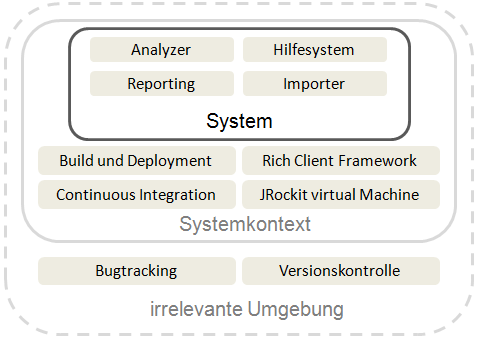
\includegraphics{images/systemumfang}
        	\caption{System und Systemkontext}
\end{figure}
\subsubsection{System}
Das System besteht aus folgenden Aspekten:
\begin{itemize}
	\item \textbf{Datenmodell, Domäne}
	\item \textbf{Parsing, Analyse}
	\item \textbf{Report, Charting}
	\item \textbf{Hilfesystem:} Dem Benutzer wird sowohl eine generelle wie auch eine kontextsensitive Hilfe\footnote{Hilfe zu aktuellen Fenstern oder Aktionen} bereitgestelt. 
	\item \textbf{Benutzerführung}
\end{itemize}

\subsubsection{Systemkontext}
Zum Systemkontext gehören folgende nicht veränderbare Komponenten:
\begin{itemize}
	\item \textbf{Versionskontrolle}
	\item \textbf{Build und Deployment, Continuous Integration:} Der Build der Software für neue Updates oder Releases wird zentral auf einem Server durchgeführt. Der Source-Code wird aus der Versionskontrolle ausgecheckt, die binären Packete werden gebildet, es wird ein für den jeweiligen Update-Mechanismus notwendiges Packet erstellt und auf den Update-Server gestellt.

	\item \textbf{Update Mechanismus:} Die Software wird in der Version 1.0 released. Anschliessend können Updates (Minor-, Major-Versionen) direkt - ohne den erneuten Download der Software - durchgeführt werden.
	\item \textbf{JRockit Virtual Machine:} Die Schnittstelle zur JRockit Virtual Machine findet über deren Log-Dateien statt. Die genaurere Beschreibung befindet sich unter \titleref{jrockitgclog}.
\end{itemize}

\subsubsection{Irrelevante Umgebung}
\begin{itemize}
	\item \textbf{Bugtracking}
\end{itemize}


\subsection{Stakeholder}
 \begin{figure}[H]
  	\centering
    	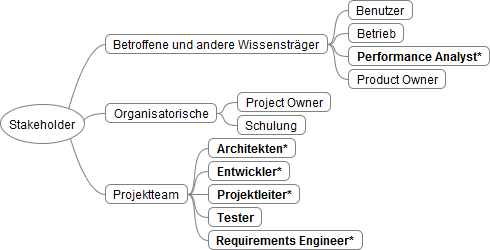
\includegraphics[width=15cm]{images/stakeholder_analyse}
        	\caption{Übersicht der Stakeholder}
\end{figure}

\subsection{Glossar}
Das Glossar befindet sich auf Seite \pageref{glossar}. 
\subsection{Referenzen}
Die Referenzen innerhalb des Abschnitts \titleref{anforderungsanalyse} befinden sich im Abschnitt Literaturverzeichnis.
\subsection{Übersicht}
Im Abschnitt \titleref{allgemeine_uebersicht} gibt es eine Beschreibung zu Architektur, Systemfunktionalität in Form eines Use-Case Diagramms, Nutzer und Zielgruppen sowie der Annahmen. 

\section{Allgemeine Übersicht}\label{allgemeine_uebersicht}
\subsection{Architekturbeschreibung}
Die Software wird als Plugin für eine Entwicklungsumgebung zur Verfügung gestellt. Der Entwickler ist in Besitz der Entwicklungsumgebung\footnote{entweder Eclipse oder Netbeans}, und kann von da durch Angabe der Update-Seite\footnote{Normalerweise werden die Software-Packete zusammen mit wenigen Meta-Informationen auf eine Update-Seite kopiert, um von da vom jeweiligen Update-Manager installiert zu werden.} als zusätzliche Funktionalität integriert werden. Ab diesem Zeitpunkt läuft die Applikation respektive das Plugin auch im offline Modus. Auch für die Analyse des Garbage Collection Logs wird durch die Applikation keine Verbindung nach aussen aufgebaut. Vorstellbare Protokolle für den Transfer der Log-Dateien - die auf dem auszuwertenden System generiert werden - sind beispielsweise FTP, SFTP, Mail, etc. Die Applikation soll für möglichst viele Betriebssysteme verfügbar sein (siehe \titleref{req_plattformunabhaengig} S. \pageref{req_plattformunabhaengig}).
\subsection{Systemfunktionalität}\label{systemfunktionalitaet}
 \begin{figure}[H]
  	\centering
    	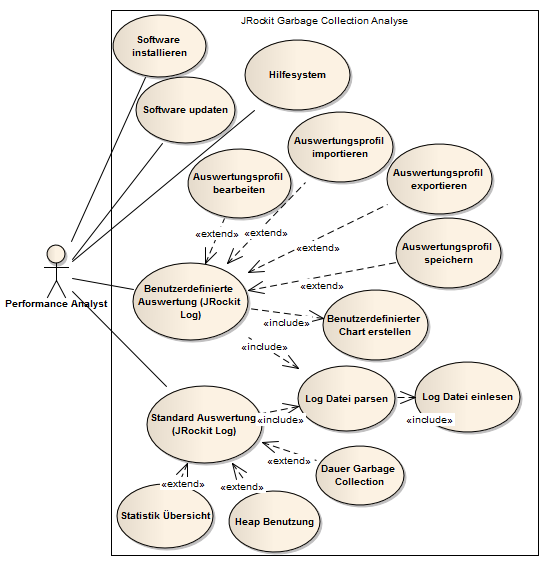
\includegraphics[width=15cm]{images/anforderungen_use-case}
        	\caption{Systemfunktionalität als Use-Case-Diagramm}
\end{figure}
\subsection{Nutzer und Zielgruppen}
\subsubsection{Performance Engineers}
Normalerweise Software Entwickler die viel Erfahrung, Wissen, Fähigkeiten haben und über die entsprechenden Werkzeuge verfügen, um Performance-Problemen von Anwendungen auf den Grund zu gehen. Dabei handelt es sich nicht nur um Wissen im Bereich der Softwareentwicklung, sondern auch im Bereich des Servers (Speicher Management, etc.), und des Betriebssystems (I/O\footnote{IO steht für Input/Output und betrifft Netzwerk wie auch Harddisk}, etc.). Durch ihr breites Wissen sind sie mit der Unterstützung von Charts, Statistiken und Reports oft sehr schnell in der Lage, Ursache eines Performance Engpasses zu finden.

\subsubsection{Java Entwickler}
Im Gegensatz zu Performance Engineers beschäftigen sich Java Entwickler vorallem mit der Entwicklung von Anwendungen und verfügen nicht direkt über Knowhow im Bereich der Performance Analyse. Als gut ausgebildete Ingenieure sind sie aber mit Hilfe von Werkzeugen und Dokumentation in der Lage, Performance Problemen innert nützlicher First auf den Grund zu gehen.

\subsection{Randbedingungen}
\subsection{Annahmen}
\section{Anforderungen}
\subsection{Funktionale Anforderungen}
Dieser Abschnitt spezifiziert die auf Seite \pageref{systemfunktionalitaet} unter \titleref{systemfunktionalitaet} im Diagramm aufgezeigten Use-Cases. Als Grundlage dient die Schablone zur Use-Case-Spezifikation in \cite[S. 78-79]{pohl2010basiswissen}.
\begin{landscape}
\section{Funktionale Anforderungen}
Aus den im Abschnitt \titleref{use_cases} definierten Anforderungen ergibt sich die abschliessende Liste der funktionalen Anforderungen:
\begin{longtable}{|p{1.8cm}|p{0.7cm}|p{2.5cm}|p{5cm}|p{1.6cm}|p{4cm}|p{0.9cm}|}
    \hline
   \textbf{Identifik.} & \textbf{Vers.}& \textbf{Titel} & \textbf{Beschreibung} & \textbf{Use Case} & \textbf{Abnahmekriter.} &\textbf{Prio.}\\\hline

   FRQ-01 & 1.0 & Installation & Software muss als Erweiterung in der Entwicklungsumgebung\footnote{Die Wahl der Entwicklungsumgebung respektive des Frameworks befindet sich im Abschnitt \titleref{selection_rcp_fw}.} installiert werden können.  & UC-01 & Entwickler mit durchschnittlichen Kenntnissen benötigen für die Installation in eine bestehende Entwicklungsumgebung dauert weniger als 5 Minuten. & gross  \\\hline

   FRQ-02 & 1.0 & Updaten & Die Software kann mit geringem Aufwand aktualisiert werden. & UC-02 & Entwickler mit durchschnittlichen Kenntnissen für den Update weniger als 3 Minuten. & mittel  \\\hline

  FRQ-03 & 1.0 & Garbage Collection Logdatei importieren & Logdateien können importiert werden und werden anschliessend in einem Fenster dargestellt. & UC-03 & - & gross  \\\hline

 FRQ-03.1 & 1.0 & Importierte Dateien speichern & Informationen über importierte Logdateien werden gespeichert und bleiben über die Zeit der Benutzersession bestehen.& UC-03.1 & - & gross  \\\hline

  FRQ-04 & 1.0 & Garbage Collection Logdatei einlesen & Geöffnete Garbage Collection Logdateien werden ins Memory gelesen. & UC-04 & Der Einleseprozess bei einer Datei mit 100000 Zeilen dauert weniger als 2 Sekunden. & gross  \\\hline

  FRQ-05 & 1.0 & Garbage Collection Logdatei parsen & Die eingelesenen JRockit Garbage Collection Logdatei wird geparst. Aus den Daten wird ein Domänenmodell aufgebaut.& UC-05 & Das Parsen einer Logdatei mit 100000 Zeilen dauert nicht länger als 8 Sekunden. & gross  \\\hline

   FRQ-06 & 1.0 & Standardauswert-ung anzeigen & Der Benutzer kann eine vordefinierte Anzeige öffnen. & UC-06 & - & gross \\\hline

   FRQ-06.1 & 1.0 & Anzeige Übersicht Garbage Collection & Der erste Tab des Analysefensters zeigt die aggregierten Daten der Garbage Collection. & UC-06.1 & Die Genauigkeit der berechneten und angezeigten Werte ist mindestens ein Zehntel (0.1). & gross \\\hline

   FRQ-06.2 & 1.0 & Anzeige Heap Benutzung & Der zweite Tab des Analysefensters zeigt den Speicherbedarf über die Zeit. & UC-06.2 & Die Genauigkeit der berechneten und angezeigten Werte ist mindestens ein Zehntel (0.1). & gross 
 \\\hline

   FRQ-06.3 & 1.0 & Anzeige Dauer Garbage Collection & Der dritte Tab des Analysefensters zeigt die Dauer der einzelnen Garbage Collections über die Zeit. & UC-06.3 & Die Genauigkeit der berechneten und angezeigten Werte ist mindestens ein Zehntel (0.1). & mittel 
 \\\hline

   FRQ-07 & 1.0 & Profil (Benutzerdefinierte Auswertung) erstellen & Benutzer kann Profil erstellen, um anschliessend darin benutzerdefinierte Charts zu erstellen.& UC-B07 & - & klein \\\hline

   FRQ-07.1 & 1.0 & Chart definieren für Profil & Für ein erstelltes Profil kann der Benutzer aus den Log-Daten ein eigenes Chart definieren. & UC-B07.1 & - & klein \\\hline

   FRQ-07.2 & 1.0 & Profil speichern & Definiertes Profil wird automatisch gespeichert und bleibt über die Dauer der Sitzung bestehen. & UC-07.2 & - & klein \\\hline

  FRQ-07.3 & 1.0 & Profil exportieren & Profil kann in Textdatei exportiert werden. & UC-07.3 & - & klein \\\hline

  FRQ-07.4 & 1.0 & Profil importieren & Profil kann aus Textdatei importiert werden. & UC-07.4 & - & klein \\\hline

  FRQ-08 & 1.0 & Hilfesystem &  Dem Benutzer werden eine indexbasierte und eine kontextsensitive Hilfe zur Verfügung gestellt. & UC-08 & Die Hilfe ist in Deutsch und Englisch verfügbar. & klein \\\hline
\caption{Funktionale Anforderungen}
\end{longtable}
\end{landscape}

\begin{landscape}
\section{Qualitätsanforderungen}
\subsection{Software}
\begin{longtable}{|p{1.8cm}|p{0.7cm}|p{2.5cm}|p{7cm}|p{4cm}|p{0.9cm}|}
    \hline
   \textbf{Identifik.} & \textbf{Vers.}& \textbf{Titel} & \textbf{Beschreibung} & \textbf{Abnahmekriter.} &\textbf{Prio.}\\\hline
   QRQ-S-01 & 1.0 & Erweiterbarkeit & Nebst der Analyse von Garbage Collection Logs der JRockit Virtual Machine sollen später auch andere Formate unterstützt sein. & Erweiterung um ein weiteres Logformat soll den Aufwand von 5 PT\footnote{Personentage} nicht überschreiten. & mittel \\\hline
   QRQ-S-02 & 1.0 & Testabdeckung & Um den langfristigen Erfolg dieser Software zu gewährleisten muss eine entsprechende Testabdeckung vorhanden sein - dies um insbesondere die Regression zu vermeiden. & Angestrebte Test-Coverage: 80\% & klein \\\hline
  QRQ-S-03 & 1.0 & Internationali-sierung & Die Sprachelemente der Software (Labels, Titel, Texte) werden als Ressourcen definiert, was die spätere Erweiterung ermöglicht. & - & klein\\\hline

   QRQ-S-04 & 1.0 & Usability & Schnelles Einlesen von grossen Dateien, Benutzerfeedback über ein Progressbar (Monitor).  & Der Import einer Log-Datei von 100000 Zeilen dauert kürzer als 10 Sekunden. Dem Benutzer wird ein Monitor bereitgestellt.&mittel \\\hline

  QRQ-S-05 & 1.0 & Korrektheit (angezeigte Werte) & Die berechneten und angezeigten Werte sind exakt. & berechnete und angezeigte Werte haben eine Genauigkeit von mindestens einem Zehntel (0.1). & gross\\\hline
\end{longtable}
\subsection{Basisframework}\label{anforderungen_framework}
\begin{longtable}{|p{1.8cm}|p{0.7cm}|p{2.5cm}|p{7cm}|p{4cm}|p{0.9cm}|}\hline
   \textbf{Identifik.} & \textbf{Vers.}& \textbf{Titel} & \textbf{Beschreibung} & \textbf{Abnahmekriter.} &\textbf{Prio.}\\\hline
   QRQ-F-01 & 1.0 & Verbreitung & Die Software wird als Erweiterung für eine Entwicklungsumgebung bereitgestellt. Die Verbreitung der Software spielt eine grosse Rolle.   & - & gross \\\hline

   QRQ-F-02 & 1.0 & Plattform-unabhängig & Software soll auf den gängigsten Betriebssystemen Windows und Apple OSX laufen. &  Framework läuft auf den Plattformen Windows und Mac OSX. & gross \\\hline

   QRQ-F-03 & 1.0 & Lokalisation & Framework muss Unterstützung für Lokalisation bereitstellen. & Framework bietet Unterstützung für die Mehrsprachigkeit. &klein \\\hline

   QRQ-F-04 & 1.0 & Modularisierung & Framework muss Unterstützung für Modularisierung bieten, damit die Software in unterschiedliche Komponenten aufgeteilt werden kann (siehe Erweiterbarkeit QRQ-S-01). & Framework bietet Unterstützung für Modularisierung.&mittel \\\hline

   FRQ-F-05 & 1.0 & Offline Betriebsmodus & Der Anwender soll die Software auch im Offline-Modus\footnote{Auf einem Computer der sich nicht am Netz befindet.} benutzen können. & Eigenständige Software, keine Web Applikation & gross  \\\hline

   FRQ-F-06 & 1.0 & Installation als Erweiterung& Software wird als Erweiterung in einer Entwicklungsumgebung installiert. & - & gross  \\\hline

    \caption{Qualitätsanforderungen Basisframework}
\end{longtable}
\end{landscape}





\subsection{Qualitätsanforderungen}
\subsubsection{Erweiterbarkeit}
\subsubsection{Verteilbarkeit}
\subsubsection{Testabdeckung}
\subsubsection{Plattformunabhängigkeit}\label{req_plattformunabhaengig}
\subsubsection{Internationalisierung}


